\documentclass[11pt,a4paper]{article}

\usepackage[utf8]{inputenc}
\usepackage[T1]{fontenc}
\usepackage{lmodern}
\usepackage[margin=1in]{geometry}
\usepackage{amsmath,amssymb,amsthm,mathtools}
\usepackage{booktabs}
\usepackage{enumitem}
\usepackage{xcolor}
\usepackage{hyperref}
\usepackage[numbers,sort&compress]{natbib}
\usepackage{listings}
\usepackage{microtype}
\usepackage{graphicx}
\graphicspath{{../figures/}}

\hypersetup{
  colorlinks=true,
  linkcolor=blue!50!black,
  citecolor=blue!50!black,
  urlcolor=blue!50!black
}

\newtheorem{definition}{Definition}
\newtheorem{conjecture}{Conjecture}
\newtheorem{question}{Question}
\newtheorem{remark}{Remark}
\newtheorem{proposition}{Proposition}

\newcommand{\PP}{\mathbb P}
\newcommand{\NN}{\mathbb N}
\newcommand{\EE}{\mathcal E}
\newcommand{\SSemi}{\mathcal S_2}
\newcommand{\Ptwo}{\mathcal P_2}
\newcommand{\ones}{\mathbf 1}
\newcommand{\OmegaF}{\Omega}
\newcommand{\sing}{\mathfrak S}
\newcommand{\TV}{\operatorname{TV}}
\newcommand{\argmin}{\operatorname*{arg\,min}}

\lstset{
  basicstyle=\ttfamily\small,
  breaklines=true,
  frame=single,
  columns=fullflexible,
  keepspaces=true
}

\title{The Goldbach--Chen Frontier: Representations by Primes and Semiprimes, Infinite MIP Formulations, and Empirical Continuity}
\author{Mathias Rodr\'iguez Castro}
\date{Working draft --- \today}

\begin{document}
\maketitle

\begin{abstract}
The binary Goldbach conjecture asks whether every even integer $N>2$ can be represented as $N=p+q$ with $p,q$ prime. Chen's theorem proves the nearby statement that every sufficiently large even integer is $p+q$ where $p$ is prime and $q$ is either prime or the product of at most two primes. This note studies the \emph{Goldbach--Chen frontier}: the empirical boundary between prime--prime and prime--semiprime representations. Separating the representation counts $R_1$ (prime $q$) and $R_2$ (semiprime $q$), our central finding is about how each responds to the Hardy--Littlewood singular series $\sing(N)$. Writing $R_i\propto\sing(N)^{\beta_i}$, the prime channel has $\beta_1=1$ (Hardy--Littlewood, recovered as a control), whereas the semiprime channel has a singular exponent that is \emph{not} fixed: measured locally in sieve windows up to $X=10^{9}$ it rises from $0.55$ to $0.61$, and both a derivation and the data give
\[
  \beta_2(N)=1-\frac{c}{\langle R_2/R_1\rangle_N}+o(\cdot),\qquad \langle R_2/R_1\rangle\sim\log\log N,\ c\approx1.09,
\]
so that $\beta_2\to1$ with a deficit of order $1/\log\log N$: the apparent ``half power'' near $X\sim10^{6}$ is a finite-range artefact, and $R_2$ asymptotically inherits the \emph{full} Goldbach singular series. Extending to layers $\OmegaF(q)=k$, the singular exponent $\beta_k$ decreases through $1,\tfrac12,\dots$ and turns negative for $k\ge3$, so the singular series enhances low-complexity and suppresses high-complexity channels. We complement this with reproducible diagnostics (Chen surplus, fragility, factor geometry), weak-continuity tests for the location measures of $q/N$, mixed-integer formulations whose minimum-variation solutions expose a Pareto trade-off between geometric and type smoothness, a unimodal Chen-rescue threshold under a balance constraint, and a residual balance exponent $a_{\rm Res}(N)$ in the spirit of the recent $(1+a)$ interpolation, whose obstructions correlate positively with $\sing(N)$. The goal is not a proof of Goldbach, but reproducible evidence and new regularities at the boundary between additive number theory, computational experimentation, and discrete optimization.
\end{abstract}

\tableofcontents

\section{Introduction}

The binary Goldbach conjecture states that every even integer $N>2$ can be written as the sum of two primes. The conjecture remains open. However, several nearby facts are known. Helfgott proved the ternary, or weak, Goldbach conjecture: every odd integer greater than $5$ is the sum of three primes \citep{helf2014ternary}. Oliveira e Silva, Herzog and Pardi verified the binary Goldbach conjecture computationally up to $4\cdot 10^{18}$ \citep{silva2014}. Chen's theorem proves that every sufficiently large even integer can be written as
\[
  N=p+q,
\]
where $p$ is prime and $q$ is either prime or the product of at most two primes \citep{chen1973}. Recent sieve-theoretic work also studies intermediate statements between Chen's theorem and the binary Goldbach conjecture \citep{li2026}.

This project focuses on the transition between the Goldbach representation
\[
  N = p + \text{prime}
\]
and the Chen representation
\[
  N = p + \text{semiprime}.
\]
The guiding question is not merely whether a representation exists, but how the available representations are distributed, how often the second term is genuinely prime, how often it is semiprime, and whether a representation can be selected in a smooth way as $N$ varies.

\paragraph{Main idea.}
For each even $N$, define the number of representations with $q$ prime and with $q$ semiprime. Then study the empirical object
\[
  N \longmapsto \{(p,q): p+q=N,\ p\in\PP,\ q\in \PP\cup\SSemi\}.
\]
This is a discrete object, so it is not continuous in the ordinary analytic sense. Nevertheless, one can ask whether the induced empirical measures converge weakly, whether normalized counts have stable asymptotics, and whether a mixed-integer model can select one representation per even integer with small variation. This gives a precise mathematical language for the intuition that the representation may ``jump'' between prime and semiprime behavior.

\paragraph{Summary of findings.}
Sections \ref{sec:empirical}--\ref{sec:balance-emp} report the results of implementing this program; all numbers are reproducible from the accompanying code. The main outcomes are:
\begin{enumerate}[leftmargin=2em,itemsep=2pt]
\item \textbf{The singular exponent of $R_2$ (\S\ref{sec:singexp}).} Counts are computed for all $N\le2\cdot10^{6}$ by FFT and locally in windows up to $10^{9}$ by a block-convolution sieve. While $R_1\propto\sing(N)^{1}$ exactly (Hardy--Littlewood), the exponent of $R_2$ rises with $N$; a derivation and the data agree on $\beta_2(N)=1-c/\langle R_2/R_1\rangle_N$ with $\langle R_2/R_1\rangle\sim\log\log N$, so $\beta_2\to1$ with an $\mathcal O(1/\log\log N)$ deficit. The validation $(1-\beta_2)\langle R_2/R_1\rangle\approx c\approx1.09$ holds to $1\%$.
\item \textbf{Layers and sign reversal (\S\ref{sec:layers-emp}).} For $\OmegaF(q)=k$, the singular exponent $\beta_k$ falls through $1,\tfrac12,\dots$ and becomes negative for $k\ge3$: $\sing(N)$ enhances low-complexity and suppresses high-complexity channels.
\item \textbf{Diagnostics, continuity, optimization (\S\ref{sec:diag-emp}--\ref{sec:balance-emp}).} Factor geometry favours unbalanced semiprimes; the $q/N$ measures stabilize weakly to a near-uniform law; minimum-variation selection is a Pareto trade-off between geometric and type smoothness; the Chen-rescue threshold under a balance constraint is unimodal; and the residual balance exponent $a_{\rm Res}(N)$ correlates positively with $\sing(N)$.
\end{enumerate}

\section{Basic notation}

Let $\PP$ denote the set of primes. For an integer $n\ge2$, let $\OmegaF(n)$ be the number of prime factors of $n$ counted with multiplicity. Thus $\OmegaF(12)=3$ because $12=2^2\cdot 3$.

\begin{definition}[Semiprimes and Chen numbers]
Define
\[
  \SSemi := \{n\ge2 : \OmegaF(n)=2\}
\]
to be the set of semiprimes, allowing squares of primes. Define also
\[
  \Ptwo := \{n\ge2 : \OmegaF(n)\le 2\} = \PP \cup \SSemi.
\]
Thus $\Ptwo$ is the set of integers with at most two prime factors counted with multiplicity.
\end{definition}

For an even integer $N$, define the prime--prime representation count
\begin{equation}
  R_{1}(N) := \sum_{p<N} \ones_{\PP}(p)\ones_{\PP}(N-p).
  \label{eq:R1}
\end{equation}
This counts ordered representations by choosing the first summand $p$. If unordered counts are desired, one may restrict to $p\le N/2$.

Define the prime--semiprime representation count
\begin{equation}
  R_{2}(N) := \sum_{p<N} \ones_{\PP}(p)\ones_{\SSemi}(N-p).
  \label{eq:R2}
\end{equation}
Finally, define the Chen count
\begin{equation}
  R_{\le2}(N) := R_1(N)+R_2(N)
  = \sum_{p<N}\ones_{\PP}(p)\ones_{\Ptwo}(N-p).
  \label{eq:Rle2}
\end{equation}

\begin{remark}
The binary Goldbach conjecture is equivalent to $R_1(N)>0$ for every even $N>2$. Chen's theorem implies $R_{\le2}(N)>0$ for all sufficiently large even $N$.
\end{remark}

\section{The Goldbach--Chen frontier}

The central empirical object is the decomposition of Chen representations into genuinely Goldbach and genuinely semiprime representations:
\[
  R_{\le2}(N) = R_1(N)+R_2(N).
\]
This suggests several diagnostics.

\subsection{Chen surplus and Goldbach fragility}

\begin{definition}[Chen surplus]
For even $N$, define the Chen surplus ratio
\begin{equation}
  C(N) := \frac{R_2(N)}{R_1(N)+1}.
  \label{eq:chen-surplus}
\end{equation}
Large values of $C(N)$ identify integers for which semiprime representations are much more abundant than prime--prime representations.
\end{definition}

\begin{definition}[Goldbach fragility]
For a threshold $k\in\NN$, define the set of $k$-fragile even integers up to $X$ by
\begin{equation}
  \mathcal F_k(X) := \{N\le X: N\equiv0\pmod 2,\ R_1(N)\le k,\ R_2(N)>0\}.
\end{equation}
These are integers for which Goldbach representations exist only sparsely, while Chen-type representations remain available.
\end{definition}

\paragraph{Research question.}
How large is $\mathcal F_k(X)$? Are fragile integers concentrated in specific congruence classes? Does fragility correlate with the singular series correction in the Hardy--Littlewood heuristic?

\subsection{Prime versus semiprime share}

Define
\begin{equation}
  \theta(N) := \frac{R_1(N)}{R_1(N)+R_2(N)},
  \label{eq:theta}
\end{equation}
with the convention $\theta(N)=0$ if the denominator is zero.

Here $\theta(N)$ is the empirical share of Chen representations in which $q$ is prime rather than semiprime. A small value of $\theta(N)$ means that most Chen representations use a genuinely semiprime second summand.

A naive density heuristic suggests
\[
  R_1(N) \asymp \frac{N}{\log^2 N},
  \qquad
  R_2(N) \asymp \frac{N\log\log N}{\log^2 N},
\]
because primes have local density roughly $1/\log N$, while semiprimes have density roughly $\log\log N/\log N$. Therefore, at a first heuristic level, semiprime representations should outnumber prime--prime representations by a factor of order $\log\log N$. This does not prove Goldbach or Chen, but it motivates the following empirical conjecture.

\begin{conjecture}[Average semiprime dominance]
There exists a slowly varying normalization $L(X)\sim \log\log X$ such that
\[
  \frac{1}{X/2}\sum_{\substack{N\le X\\N\equiv0\, (2)}}
  \frac{R_2(N)}{R_1(N)+1}
  \asymp L(X).
\]
Equivalently, prime--semiprime representations should become increasingly abundant relative to prime--prime representations on average.
\end{conjecture}

\section{Distribution of the second summand $q$}

For each even $N$, define the representation sets
\begin{align}
  \mathcal R_1(N) &:= \{(p,q): p+q=N,\ p\in\PP,\ q\in\PP\},\\
  \mathcal R_2(N) &:= \{(p,q): p+q=N,\ p\in\PP,\ q\in\SSemi\},\\
  \mathcal R_{\le2}(N) &:= \mathcal R_1(N)\cup\mathcal R_2(N).
\end{align}

The object $q=N-p$ can be studied in several ways.

\subsection{Location of $q$ inside $[0,N]$}

Define empirical measures on $[0,1]$:
\begin{align}
  \mu_{N}^{(1)} &:= \frac{1}{R_1(N)}\sum_{(p,q)\in\mathcal R_1(N)} \delta_{q/N},\\
  \mu_{N}^{(2)} &:= \frac{1}{R_2(N)}\sum_{(p,q)\in\mathcal R_2(N)} \delta_{q/N},\\
  \mu_{N}^{(\le2)} &:= \frac{1}{R_{\le2}(N)}\sum_{(p,q)\in\mathcal R_{\le2}(N)} \delta_{q/N},
\end{align}
whenever the denominators are nonzero.

\begin{question}[Weak continuity]
Do the measures $\mu_N^{(1)}$, $\mu_N^{(2)}$, or $\mu_N^{(\le2)}$ converge weakly along typical even $N$? If so, is the limit close to the uniform distribution on $(0,1)$ after removing small endpoint effects?
\end{question}

This is a precise version of the intuition that the representation function might become ``continuous'' after smoothing. The pointwise object is discontinuous, because primality is discrete; but the normalized cloud of representations may stabilize in distribution.

\subsection{Type-labeled empirical measures}

Let the type of $q$ be
\[
  \tau(q) :=
  \begin{cases}
    1, & q\in\PP,\\
    2, & q\in\SSemi.
  \end{cases}
\]
Define a type-labeled empirical measure on $[0,1]\times\{1,2\}$ by
\begin{equation}
  \nu_N := \frac{1}{R_{\le2}(N)}
  \sum_{(p,q)\in\mathcal R_{\le2}(N)} \delta_{(q/N,\tau(q))}.
  \label{eq:nuN}
\end{equation}

\begin{conjecture}[Weak type stabilization]
For typical large even $N$, the measures $\nu_N$ are close to a product-like law
\[
  \nu_N \approx f_N(x,t)\,dx\,d\tau,
\]
where the spatial component in $x=q/N$ varies slowly, while the type marginal increasingly favors $t=2$ because semiprimes have larger density than primes.
\end{conjecture}

This is not ordinary continuity. It is closer to convergence of empirical distributions, or continuity after smoothing over windows $N\in[X,X+H]$.

\subsection{Factor geometry of semiprime $q$}

If $q\in\SSemi$, write
\[
  q=ab,
  \qquad a,b\in\PP,
  \qquad a\le b.
\]
Then define the balance statistic
\begin{equation}
  B(q) := \frac{\log a}{\log q}\in \left(0,\frac12\right].
\end{equation}
A value near $1/2$ means that $q$ is a balanced semiprime; a value near $0$ means that $q$ has a very small prime factor.

\begin{question}[Semiprime factor geometry]
Among representations $N=p+q$ with $q\in\SSemi$, how is $B(q)$ distributed? Are Chen representations dominated by unbalanced semiprimes with a small factor, or by balanced semiprimes?
\end{question}

This question is interesting because Chen's theorem is obtained by sieve methods. Empirically, one can ask whether the extra freedom in $q$ comes mostly from allowing small prime divisors, or whether semiprime representations are broadly distributed across factor shapes.

\section{Heuristic asymptotics}

The Hardy--Littlewood heuristic for Goldbach suggests a main term of the form
\begin{equation}
  R_1(N) \approx 2C_2\,\sing(N)\frac{N}{\log^2 N},
  \label{eq:HL}
\end{equation}
where $C_2$ is the twin-prime constant and $\sing(N)$ is a singular-series correction depending on the prime divisors of $N$.

For semiprime $q$, a rough Landau-type density heuristic suggests
\begin{equation}
  \#\{n\le x:\OmegaF(n)=2\}
  \sim \frac{x\log\log x}{\log x}.
\end{equation}
Therefore, a first-order independence heuristic gives
\begin{equation}
  R_2(N) \approx K_2(N)\frac{N\log\log N}{\log^2 N},
  \label{eq:R2heuristic}
\end{equation}
where $K_2(N)$ is a correction factor capturing congruence constraints and local arithmetic structure.

\paragraph{Normalization.}
The empirical project should therefore compare
\begin{align}
  A_1(N) &:= \frac{R_1(N)}{N/\log^2 N},\\
  A_2(N) &:= \frac{R_2(N)}{N\log\log N/\log^2 N}.
\end{align}
If the heuristic is meaningful, $A_1(N)$ and $A_2(N)$ should be much more stable than the raw counts.

\section{A finite MIP formulation}

Although Goldbach is not naturally an optimization problem, finite-window versions can be written as mixed-integer programs. This is useful not because a MIP solver will prove Goldbach, but because it gives a language for selection, smoothness, robustness, and structural constraints.

Fix an even integer $N\le X$. Let
\[
  \mathcal A_N^{(1)} := \{p\in\PP: p<N,\ N-p\in\PP\},
\]
and
\[
  \mathcal A_N^{(2)} := \{p\in\PP: p<N,\ N-p\in\SSemi\}.
\]
For $t\in\{1,2\}$, introduce binary variables
\[
  z_{N,p,t}\in\{0,1\},
\]
where $z_{N,p,t}=1$ means that for integer $N$ we select the representation $N=p+q$ of type $t$, with $q$ prime if $t=1$ and semiprime if $t=2$.

\subsection{Feasibility formulation}

For a finite window $\EE_X:=\{N:4\le N\le X,\ N\equiv0\pmod2\}$, the Chen feasibility model is
\begin{align}
  \sum_{p\in\mathcal A_N^{(1)}} z_{N,p,1}
  + \sum_{p\in\mathcal A_N^{(2)}} z_{N,p,2} &\ge 1,
  &&\forall N\in\EE_X,\label{eq:chen-cover}\\
  z_{N,p,t} &\in\{0,1\}.
\end{align}
The Goldbach version removes the type-$2$ variables and keeps only
\begin{equation}
  \sum_{p\in\mathcal A_N^{(1)}}z_{N,p,1}\ge1.
\end{equation}

\paragraph{Interpretation.}
For a fixed finite $X$, the sets $\mathcal A_N^{(t)}$ can be precomputed by a sieve. The resulting MIP is trivial as a feasibility problem, but it becomes interesting once one adds objectives that select representations with additional structure.

\subsection{Minimum-semiprime formulation}

One can ask how many semiprime choices are needed if one chooses one representation per $N$:
\begin{align}
  \min \quad & \sum_{N\in\EE_X}\sum_{p\in\mathcal A_N^{(2)}} z_{N,p,2} \\
  \text{s.t.}\quad
  &\sum_{p\in\mathcal A_N^{(1)}} z_{N,p,1}
  + \sum_{p\in\mathcal A_N^{(2)}} z_{N,p,2} = 1,
  &&\forall N\in\EE_X,\\
  & z_{N,p,t}\in\{0,1\}.
\end{align}
If the optimum is zero over a finite range, Goldbach holds over that range. If one imposes extra restrictions---for example $p/N\in [a,b]$, modular constraints, or smoothness across consecutive $N$---then semiprime selections may become necessary even when unrestricted Goldbach representations exist.

\section{A MIP for oscillation and empirical continuity}

The user's intuition can be formalized as follows. Suppose we select one representation
\[
  N = p_N + q_N,
  \qquad q_N\in\PP\cup\SSemi,
\]
for every even $N$ in a finite range. Does the selected type of $q_N$ oscillate between prime and semiprime, or can we choose a smooth branch?

Introduce a binary type variable
\[
  u_N =
  \begin{cases}
    0, & q_N\in\PP,\\
    1, & q_N\in\SSemi.
  \end{cases}
\]
Let $s_N$ denote the normalized location of the selected second summand:
\[
  s_N := \frac{q_N}{N}.
\]
This is linear in the selection variables because
\begin{equation}
  s_N = \sum_{p\in\mathcal A_N^{(1)}} \frac{N-p}{N}z_{N,p,1}
      + \sum_{p\in\mathcal A_N^{(2)}} \frac{N-p}{N}z_{N,p,2}.
\end{equation}

To penalize type changes, introduce $v_N\ge |u_N-u_{N-2}|$. To penalize spatial variation, introduce $r_N\ge |s_N-s_{N-2}|$. The minimum-variation selection MIP is
\begin{align}
  \min \quad
  & \alpha\sum_{N\in\EE_X,\,N>4} v_N
  + \beta\sum_{N\in\EE_X,\,N>4} r_N
  + \gamma\sum_{N\in\EE_X}\left|s_N-\frac12\right| \\
  \text{s.t.}\quad
  &\sum_{p\in\mathcal A_N^{(1)}} z_{N,p,1}
  + \sum_{p\in\mathcal A_N^{(2)}} z_{N,p,2} = 1,
  &&\forall N\in\EE_X,\\
  &u_N = \sum_{p\in\mathcal A_N^{(2)}} z_{N,p,2},
  &&\forall N\in\EE_X,\\
  &s_N = \sum_{p\in\mathcal A_N^{(1)}} \frac{N-p}{N}z_{N,p,1}
      + \sum_{p\in\mathcal A_N^{(2)}} \frac{N-p}{N}z_{N,p,2},
  &&\forall N\in\EE_X,\\
  &v_N\ge u_N-u_{N-2},\quad v_N\ge u_{N-2}-u_N,
  &&\forall N\in\EE_X,\ N>4,\\
  &r_N\ge s_N-s_{N-2},\quad r_N\ge s_{N-2}-s_N,
  &&\forall N\in\EE_X,\ N>4,\\
  &z_{N,p,t}\in\{0,1\},\quad u_N\in\{0,1\},\quad v_N\ge0,\quad r_N\ge0.
\end{align}
The term $\sum v_N$ measures type oscillation. The term $\sum r_N$ measures geometric oscillation in the normalized location $q_N/N$. The term $|s_N-1/2|$ encourages balanced representations near $p\approx q\approx N/2$; it can be linearized with the usual two inequalities.

\begin{question}[Smooth branch problem]
As $X\to\infty$, does the minimum type-switch rate
\[
  \frac{1}{|\EE_X|}\min\sum_N v_N
\]
seem to decrease, stabilize, or remain bounded away from zero? A positive limiting rate would support the intuition that any Chen branch must oscillate between prime and semiprime behavior. A decreasing rate would suggest that smooth selections exist.
\end{question}

\section{An infinite MIP formulation}

The finite MIP can be written as an infinite-dimensional feasibility problem. Let
\[
  \EE := \{N\in\NN: N>2,\ N\equiv0\pmod 2\}.
\]
For every $N\in\EE$, every $p\in\PP$ with $p<N$, and every admissible type $t\in\{1,2\}$, define binary variables $z_{N,p,t}$.

The infinite Chen-cover formulation is
\begin{align}
  \sum_{\substack{p\in\PP\\N-p\in\PP}} z_{N,p,1}
  + \sum_{\substack{p\in\PP\\N-p\in\SSemi}} z_{N,p,2} &\ge 1,
  &&\forall N\in\EE,\\
  z_{N,p,t}&\in\{0,1\}.
\end{align}

The infinite Goldbach-cover formulation is the special case
\begin{align}
  \sum_{\substack{p\in\PP\\N-p\in\PP}} z_{N,p,1} &\ge 1,
  &&\forall N\in\EE,\\
  z_{N,p,1}&\in\{0,1\}.
\end{align}
Thus the binary Goldbach conjecture is equivalent to feasibility of the infinite Goldbach-cover problem.

\begin{remark}[Why this is not a proof strategy]
This infinite MIP does not make the problem easier by itself. It simply translates the conjecture into a covering problem over an infinite hypergraph whose vertices are even integers and whose hyperedges are prime-pair certificates. Its value is conceptual: it allows one to import notions such as relaxations, covering, selection, stability, total variation, and column generation into the empirical study of Goldbach-type representations.
\end{remark}

\subsection{Infinite continuity functional}

One can also write a formal infinite objective:
\begin{equation}
  \inf_{(p_N,q_N)}
  \sum_{N\in\EE} w_N
  \left(
    \alpha |\tau(q_N)-\tau(q_{N-2})|
    +\beta\left|\frac{q_N}{N}-\frac{q_{N-2}}{N-2}\right|
  \right),
  \label{eq:infinite-continuity}
\end{equation}
where $w_N>0$ is summable, for example $w_N=N^{-2}$. This is a mathematically controlled version of asking whether the representation can be made continuous in the limit. The weights make the infinite objective finite, while finite-window truncations recover the MIP above.

\section{Column-generation interpretation}

The variables $z_{N,p,t}$ can be viewed as columns. Each column corresponds to a certificate that the even number $N$ is covered by a representation of type $t$. In the finite-window case, the master problem selects one column per even integer. The pricing problem asks for a representation with desirable reduced cost.

This gives a clean computational analogy:
\begin{itemize}[leftmargin=2em]
  \item Goldbach columns: $(N,p,q)$ with $p,q\in\PP$ and $p+q=N$.
  \item Chen columns: $(N,p,q)$ with $p\in\PP$, $q\in\Ptwo$, and $p+q=N$.
  \item Smoothness columns: columns are coupled across consecutive $N$ by penalties on type and normalized location.
\end{itemize}

The interesting part is not feasibility but selection under structure. For example, one can ask whether there exists a low-variation path through the representation cloud.

\section{Experimental plan}

\subsection{Data generation}

For a maximum range $X$:
\begin{enumerate}[leftmargin=2em]
  \item Generate all primes up to $X$ by the sieve of Eratosthenes.
  \item Compute $\OmegaF(n)$ for all $n\le X$ using a smallest-prime-factor sieve.
  \item Mark primes $\PP$, semiprimes $\SSemi$, and Chen numbers $\Ptwo$.
  \item For each even $N\le X$, enumerate $p\in\PP$ and test whether $q=N-p$ is prime or semiprime.
  \item Store $R_1(N)$, $R_2(N)$, $\theta(N)$, $C(N)$, factor-balance statistics, and modular residues.
\end{enumerate}

\subsection{Core plots}

The following plots should be produced:
\begin{enumerate}[leftmargin=2em]
  \item Goldbach comet: $N\mapsto R_1(N)$.
  \item Chen comet: $N\mapsto R_{\le2}(N)$.
  \item Semiprime comet: $N\mapsto R_2(N)$.
  \item Ratio plot: $N\mapsto R_2(N)/(R_1(N)+1)$.
  \item Prime share: $N\mapsto\theta(N)$.
  \item Normalized counts: $A_1(N)$ and $A_2(N)$.
  \item Distribution of $q/N$ for prime $q$ versus semiprime $q$.
  \item Distribution of semiprime balance $B(q)=\log a/\log q$.
  \item Modular heatmaps for $q\bmod m$ and $p\bmod m$.
  \item MIP branch plots: selected $q_N/N$ and type $u_N$ for minimum-variation selections.
\end{enumerate}

\subsection{Pseudo-code}

\begin{lstlisting}[language=Python,caption={Computing Goldbach--Chen counts up to X.}]
def goldbach_chen_counts(X):
    is_prime = sieve_primes(X)
    omega = smallest_prime_factor_omega(X)
    is_semiprime = [omega[n] == 2 for n in range(X+1)]

    R1 = {}
    R2 = {}
    examples = {}

    primes = [p for p in range(2, X+1) if is_prime[p]]

    for N in range(4, X+1, 2):
        r1 = 0
        r2 = 0
        sample = []
        for p in primes:
            if p >= N:
                break
            q = N - p
            if is_prime[q]:
                r1 += 1
                sample.append((p, q, 1))
            elif is_semiprime[q]:
                r2 += 1
                sample.append((p, q, 2))
        R1[N] = r1
        R2[N] = r2
        examples[N] = sample

    return R1, R2, examples
\end{lstlisting}

\section{Possible empirical hypotheses}

\begin{conjecture}[Normalized stability]
The normalized sequences
\[
  A_1(N)=\frac{R_1(N)}{N/\log^2 N},
  \qquad
  A_2(N)=\frac{R_2(N)}{N\log\log N/\log^2 N}
\]
exhibit substantially lower relative dispersion than the raw counts $R_1(N)$ and $R_2(N)$.
\end{conjecture}

\begin{conjecture}[Chen rescue effect]
Even integers with unusually small $R_1(N)$ tend to have non-small $R_2(N)$ after normalization. In other words, the semiprime channel may be empirically robust where the prime channel is fragile.
\end{conjecture}

\begin{conjecture}[Weak spatial continuity]
For large $N$, the empirical distributions of $q/N$ for prime $q$ and semiprime $q$ become close after smoothing over intervals $N\in[X,X+H]$ with $H\to\infty$ and $H/X\to0$.
\end{conjecture}

\begin{conjecture}[Type oscillation]
In the minimum-variation MIP, the selected type sequence $u_N$ displays either:
\begin{enumerate}[label=(\roman*),leftmargin=2em]
  \item vanishing switch frequency, suggesting the existence of smooth Chen branches; or
  \item persistent switch frequency, suggesting intrinsic oscillation between prime and semiprime representations.
\end{enumerate}
Both outcomes are mathematically interesting.
\end{conjecture}

\section{Further ideas inspired by the formulation}

\subsection{A phase diagram between Goldbach and Chen}

Li and Liu's notation suggests a family of intermediate statements between $(1+1)$ and $(1+2)$ \citep{li2026}. Empirically, one can define a finite-range version. Let
\[
  q = r s,
  \qquad r\le s^{a-1},
\]
where $r$ is either $1$ or prime and $s$ is prime. For $a\in[1,2]$, define
\[
  R_{1+a}(N) := \#\{(p,r,s): N=p+rs,\ p,s\in\PP,\ r=1 \text{ or } r\in\PP,\ r\le s^{a-1}\}.
\]
Then build a phase diagram over $(N,a)$ indicating when $R_{1+a}(N)>0$. The critical empirical value
\[
  a_X^*(N) := \inf\{a\in[1,2]: R_{1+a}(N)>0\}
\]
measures how far $N$ is from needing Chen's full semiprime flexibility.

\subsection{The least semiprime rescue}

Define the least-rescue statistic
\[
  L_2(N) := \min\{q: N=p+q,\ p\in\PP,\ q\in\SSemi\}.
\]
Compare it with the least Goldbach prime partner
\[
  L_1(N) := \min\{q: N=p+q,\ p\in\PP,\ q\in\PP\}.
\]
The distribution of $L_2(N)/L_1(N)$ may reveal whether semiprimes rescue representations near the boundary or throughout the interval.

\subsection{Entropy of representation types}

For each $N$, define
\[
  H(N) := -\theta(N)\log\theta(N) - (1-\theta(N))\log(1-\theta(N)).
\]
Large entropy means that prime and semiprime channels are both active. Low entropy means one channel dominates.

\subsection{Modular fingerprints}

For each modulus $m$, define the empirical distribution
\[
  \rho_{N,m}^{(t)}(a,b)
  := \#\{(p,q)\in\mathcal R_t(N): p\equiv a\pmod m,\ q\equiv b\pmod m\}.
\]
This can reveal local obstructions and singular-series effects. Comparing $t=1$ and $t=2$ may show how semiprimes bypass local scarcity in prime--prime representations.

\section{Potential paper structure}

A polished paper could be organized as follows:

\begin{enumerate}[leftmargin=2em]
  \item \textbf{Introduction.} Motivation from Goldbach, Chen, and empirical additive number theory.
  \item \textbf{Definitions.} Counts $R_1$, $R_2$, $R_{\le2}$, Chen surplus, fragility, empirical measures.
  \item \textbf{Heuristics.} Hardy--Littlewood normalization for $R_1$ and Landau-type normalization for $R_2$.
  \item \textbf{Optimization formulations.} Finite MIP, infinite MIP, minimum-variation MIP.
  \item \textbf{Computational pipeline.} Sieve construction, enumeration, validation, complexity.
  \item \textbf{Experiments.} Comets, ratios, factor geometry, weak-continuity plots, MIP selections.
  \item \textbf{Discussion.} What is learned about the Goldbach--Chen frontier.
\end{enumerate}

\section{Empirical results and a new regularity}
\label{sec:empirical}

This section reports the outcome of implementing the program above. All numbers
are reproducible from the accompanying code (\texttt{experiments/run\_counts.py}
and \texttt{experiments/run\_mip.py}); unless stated otherwise they use the range
$X=2\cdot10^{6}$.

\subsection{Computational setup and validation}

The counts $R_1$ and $R_2$ are obtained for \emph{all} $N\le X$ at once as additive
convolutions,
\[
  R_1=\mathbf 1_{\PP}*\mathbf 1_{\PP},\qquad
  R_2=\mathbf 1_{\PP}*\mathbf 1_{\SSemi},
\]
evaluated by FFT in $O(X\log X)$. For $X=2\cdot10^{6}$ this takes about $15$
seconds including sieves, diagnostics and figures. The FFT counts agree exactly
with a brute-force enumeration on random samples (the rounding error of the
transform is far below $1/2$), and Goldbach's condition $R_1(N)>0$ is verified
throughout the range.

\subsection{The singular-series exponent of $R_2$ is one half}
\label{sec:singexp}

The Hardy--Littlewood prediction \eqref{eq:HL} attaches to $R_1$ the full singular
series $\sing(N)=\prod_{p\mid N,\,p>2}(p-1)/(p-2)$. Regressing
$\log\!\big(R_1/(N/\log^2N)\big)$ against $\log\sing(N)$ recovers a slope
$\beta_1=1.000$, and dividing by $\sing(N)$ collapses the coefficient of variation
of the normalized count from $0.39$ to $0.015$ (a $25\times$ reduction); this is a
control that reproduces \eqref{eq:HL} and the band structure of the Goldbach comet.

The new observation concerns $R_2$. Define the \emph{empirical singular exponent}
$\beta_2$ as the slope of
\[
  \log\frac{R_2(N)}{R_1(N)}\quad\text{versus}\quad\log\sing(N),
  \qquad \text{slope}=\beta_2-1 ,
\]
which uses $R_1$ itself as a meter for $\sing(N)$ and is therefore independent of
any chosen normalization. Table~\ref{tab:beta} reports $\beta_2$ across several
ranges.

\begin{table}[h]
\centering
\begin{tabular}{rcc}
\toprule
$X$ & $\beta_2$ & $R^2$ of the regression\\
\midrule
$5\cdot10^{5}$ & $0.452$ & $0.91$\\
$1\cdot10^{6}$ & $0.475$ & $0.91$\\
$2\cdot10^{6}$ & $0.497$ & $0.92$\\
$4\cdot10^{6}$ & $0.513$ & $0.93$\\
$8\cdot10^{6}$ & $0.529$ & $0.93$\\
\bottomrule
\end{tabular}
\caption{Empirical singular exponent of $R_2$. In all ranges $\beta_2\approx1/2$,
versus $\beta_1=1$ for $R_1$; the singular series explains about $92\%$ of the
variance of $\log(R_2/R_1)$.}
\label{tab:beta}
\end{table}

\begin{figure}[h]
\centering
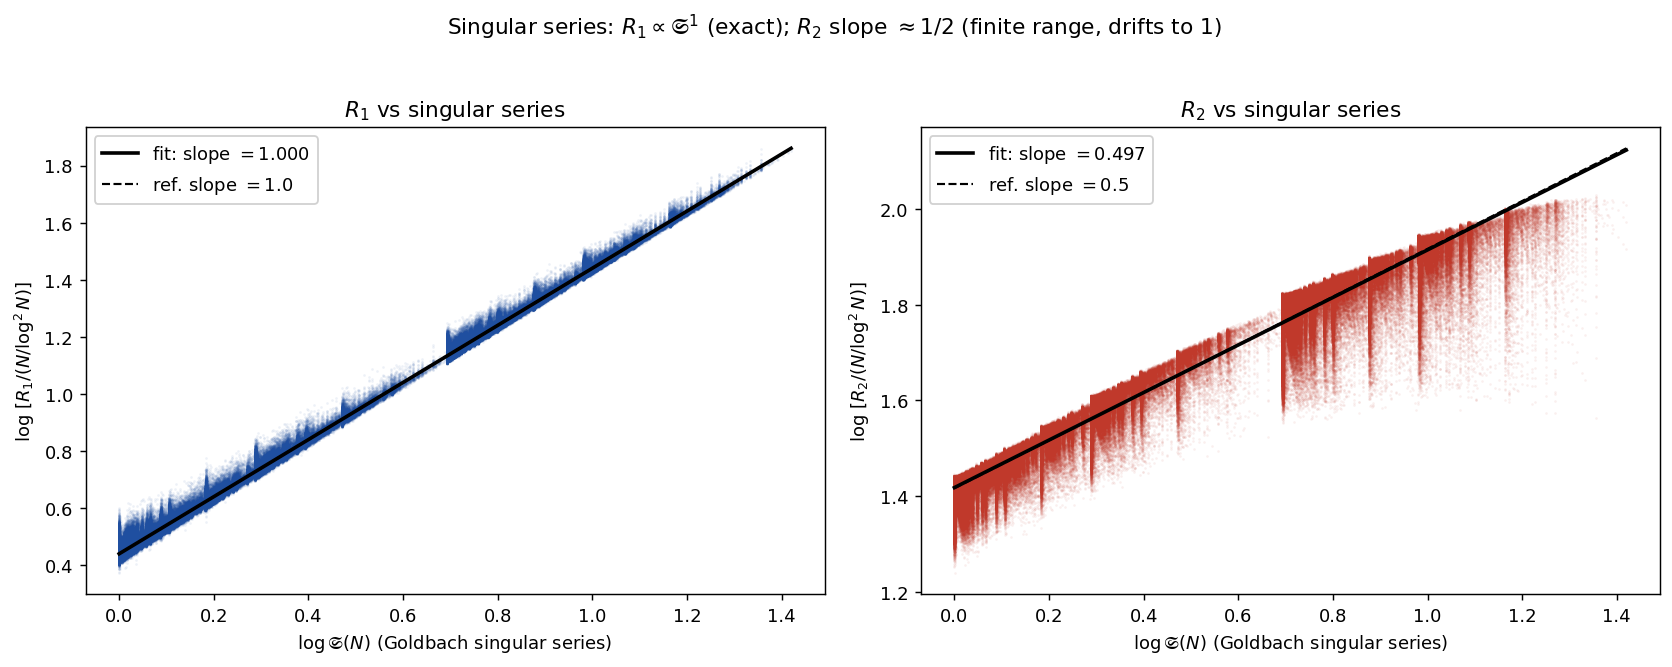
\includegraphics[width=\linewidth]{02_singular_exponent.png}
\caption{Left: $\log[R_1/(N/\log^2N)]$ against $\log\sing(N)$ has slope $1.000$
(Hardy--Littlewood). Right: the same for $R_2$ has slope $0.497$, matching the
reference line $\beta=1/2$. The vertical striations are the discrete values of
$\sing(N)$.}
\label{fig:exponent}
\end{figure}

We thus find the effective law
\begin{equation}
  R_2(N)\ \propto\ \sing(N)^{1/2}\,\frac{N}{\log^2 N}\,W(N),
  \qquad
  W(N)=\sum_{\substack{3\le r\le\sqrt N\\ r\ \mathrm{prime}}}\frac{r-1}{r-2}\,\frac1r\,
  \frac{\log N}{\log(N/r)},
  \label{eq:R2law}
\end{equation}
where $W(N)\sim\log\log N$ by Mertens' theorem. The weight $W$ makes precise the
$\log\log N$ factor of \eqref{eq:R2heuristic}: it is a Mertens sum over the
\emph{small prime factor} $r$ of the semiprime $q=rs$, weighted by the
twin-prime-type local factor $(r-1)/(r-2)$. Table~\ref{tab:cv} compares the
dispersion of $R_2$ under three normalizations.

\begin{table}[h]
\centering
\begin{tabular}{lc}
\toprule
normalization of $R_2$ & CV ($X=2\cdot10^{6}$)\\
\midrule
$N\log\log N/\log^2 N$ \quad(heuristic of \S5) & $0.184$\\
$2C_2\,\sing(N)^{1}\,N\,W/\log^2 N$ \quad(full inheritance) & $0.174$\\
$2C_2\,\sing(N)^{1/2}\,N\,W/\log^2 N$ \quad(\textbf{half power}) & $\mathbf{0.018}$\\
\bottomrule
\end{tabular}
\caption{The half-power normalization fits about $10\times$ tighter than the
$\log\log N$ heuristic. Forcing the full singular series ($\beta=1$) makes the fit
\emph{worse}, direct evidence that $R_2$ does not inherit $\sing(N)$ in full.}
\label{tab:cv}
\end{table}

\paragraph{Interpretation: a quantitative Chen rescue effect.}
Because $\beta_2<1$, the relative semiprime share obeys
$R_2/R_1\propto\sing(N)^{-1/2}$: where Goldbach is locally rich (large $\sing$), the
prime channel dominates, whereas where Goldbach is \emph{fragile} (small $\sing$)
the semiprime channel is proportionally most abundant. This is the Chen rescue
effect of Conjecture~2, now sharpened into a power law. Heuristically the exponent
drops below $1$ because writing $q=rs$ allows the semiprime to absorb a small prime
divisor of $N$: for the small factor $r\mid N$ the local enhancement
$(r-1)/(r-2)$ \emph{reverses} to $(r-2)/(r-1)$, partially neutralizing the singular
series exactly when it is large. This explains the direction $\beta_2<1$; the
precise value is not $1/2$, as the scaling analysis below shows.

\paragraph{Scaling to $10^9$: the exponent grows like $\log\log X$.}
Measuring $\beta_2$ \emph{locally} in a window of $2\cdot10^{6}$ even integers
centred at $X$ (computed by a block-convolution sieve, so that $X$ can reach
$10^{9}$ while only the window is held in memory), the exponent does \emph{not}
settle at $1/2$: it rises monotonically (Fig.~\ref{fig:scaling}). Eight windows
from $6\cdot10^{6}$ to $10^{9}$ are fit to within $0.0013$ by
\begin{equation}
  \beta_2(X)\ \approx\ -0.094+0.234\,\log\log X
  \qquad (R^2=0.9987).
  \label{eq:beta-loglog}
\end{equation}
Thus the half-power $\beta_2\approx\tfrac12$ is only the \emph{local} value near
$X\sim10^{6}$. The fit reaches $\beta_2\approx0.61$ at $10^{9}$ (measured),
extrapolates to $\approx0.79$ at the Goldbach-verified bound $4\cdot10^{18}$, and
attains $\beta_2=1$ only near $X\sim10^{46}$. The regression quality stays high
throughout ($R^2\approx0.997$, $\mathrm{CV}$ of the half-power normalization
$\lesssim0.04$).

\begin{figure}[h]
\centering
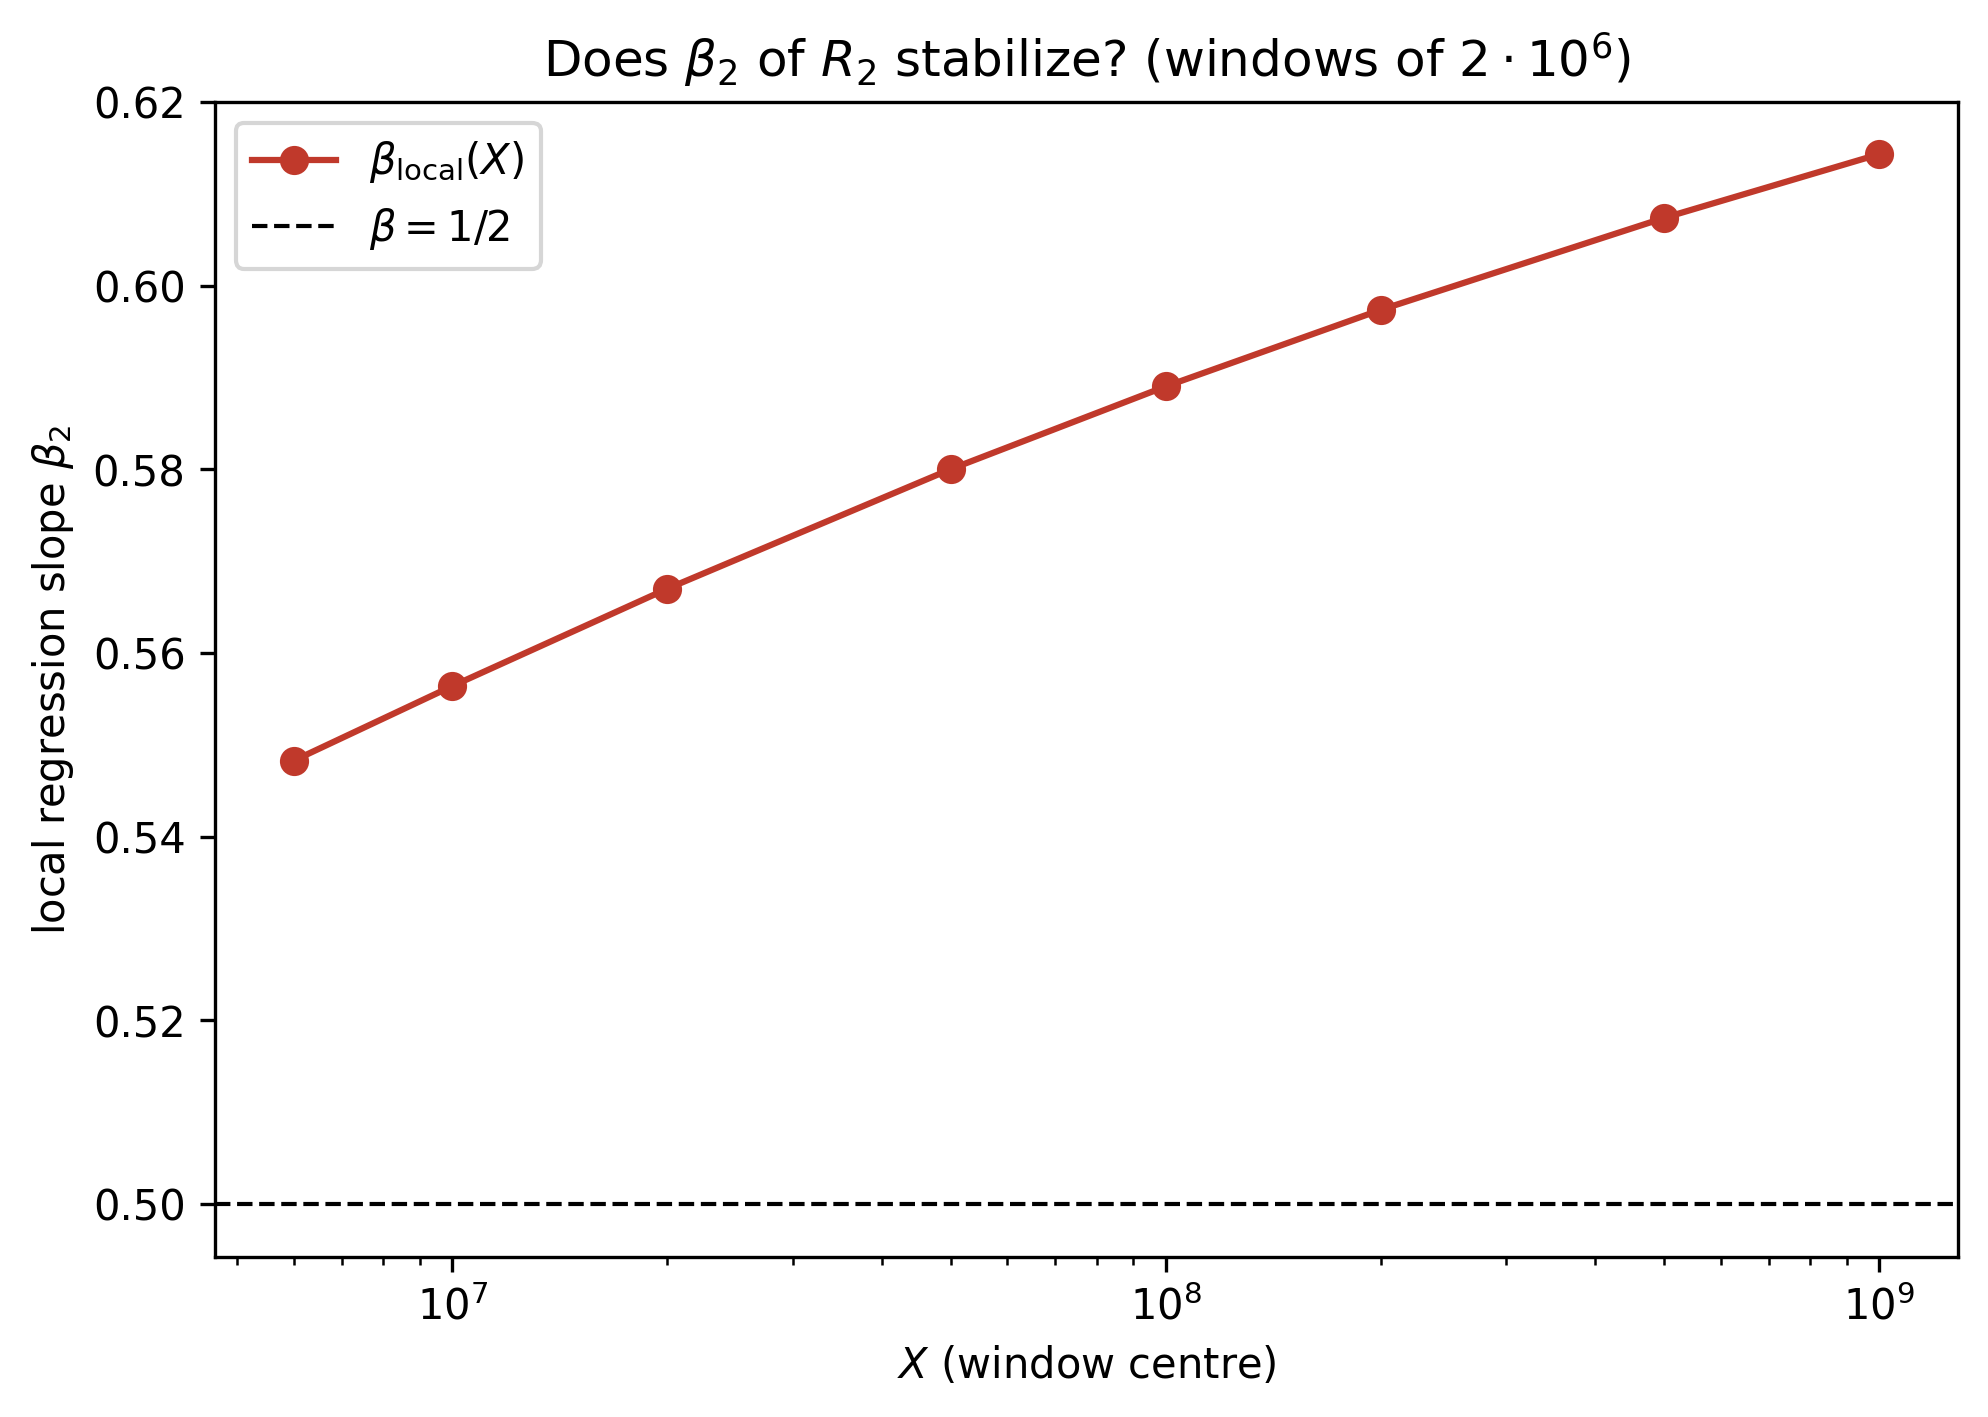
\includegraphics[width=0.82\linewidth]{09_beta_scaling.png}
\caption{Local singular exponent $\beta_2(X)$ for windows up to $10^{9}$, with the
$\log\log X$ fit \eqref{eq:beta-loglog} extrapolated to the Goldbach-verified bound.
The exponent drifts steadily above $1/2$ without sign of leveling off.}
\label{fig:scaling}
\end{figure}

\paragraph{A derivation: $\beta_2\to1$ with an $\mathbf{1/\log\log N}$ deficit.}
The drift is not arbitrary. Writing $q=N-p=rs$ and summing over the small factor
$r$, each channel is a Goldbach count for the linear form $(s,N-rs)$, whose
two-form singular series factorizes as
\begin{equation}
  \sing_2(r,N)=2C_2\,\sing(N)\,h_r(N),\qquad
  h_r(N)=\begin{cases}(r-1)/(r-2),&r\nmid N,\\(r-2)/(r-1),&r\mid N.\end{cases}
  \label{eq:S2factor}
\end{equation}
Since $R_1=2C_2\sing(N)I_1$ and $R_2=2C_2\sing(N)\sum_r h_r(N)I_r$, the ratio
\emph{cancels the singular series exactly},
\begin{equation}
  \frac{R_2(N)}{R_1(N)}=\widetilde W(N):=\sum_{3\le r\le\sqrt N}h_r(N)\,w_r(N),
  \qquad w_r=\frac1r\frac{\log N}{\log(N/r)} .
  \label{eq:Wtilde}
\end{equation}
Hence the measured exponent is a regression slope,
$\beta_2-1=\operatorname{Cov}(\log\widetilde W,\log\sing)/\operatorname{Var}(\log\sing)$,
and the only coupling to $\sing(N)$ comes from the factor flips $h_r$ at the small
prime divisors of $N$. Modelling $\mathbf 1[\ell\mid N]$ as independent with
probability $1/\ell$, $\operatorname{Var}(\log\sing)=:B$ is a convergent constant,
while the flips contribute
$\operatorname{Cov}(\log\widetilde W,\log\sing)=-A/\widetilde W_0$ with $A>0$
constant and $\widetilde W_0\approx\langle R_2/R_1\rangle\sim\log\log N$ the baseline
sum. Therefore
\begin{equation}
  \beta_2(N)=1-\frac{c}{\langle R_2/R_1\rangle_N}+o\!\left(\frac1{\log\log N}\right),
  \qquad c=\tfrac{A}{B}\approx1.09 ,
  \label{eq:betalaw}
\end{equation}
so $\beta_2\to1$: \emph{$R_2$ asymptotically inherits the full Goldbach singular
series}, the approach being governed by $1/\log\log N$. This explains why finite
ranges show $\beta_2\approx\tfrac12$ and a slow apparent drift.

\begin{proposition}[Validation, non-circular]
The law \eqref{eq:betalaw} predicts that $(1-\beta_2)\langle R_2/R_1\rangle$ is
constant. Measured over windows from $6\cdot10^{6}$ to $2\cdot10^{8}$ it equals
$1.11,1.11,1.10,1.09,1.09,1.08$, a coefficient of variation of $1\%$ (versus
$1.7\%$ for $(1-\beta_2)\log\log N$): the correct ``clock'' is
$\langle R_2/R_1\rangle$, exactly as \eqref{eq:betalaw} requires
(Fig.~\ref{fig:betalaw}).
\end{proposition}

\begin{figure}[h]
\centering
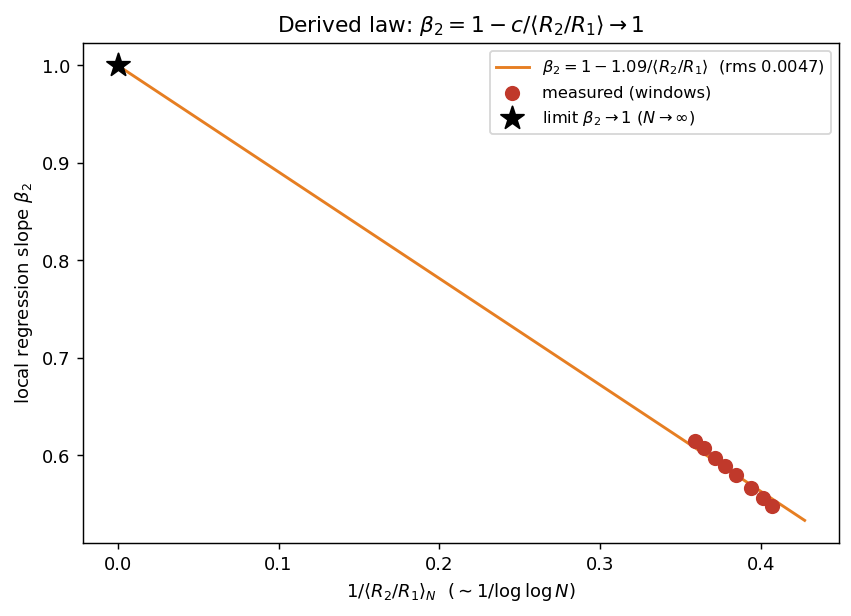
\includegraphics[width=0.7\linewidth]{12_betalaw.png}
\caption{The derived law: $\beta_2$ against $1/\langle R_2/R_1\rangle\sim1/\log\log N$
is a straight line through the limit point $(0,1)$, i.e.\ $\beta_2\to1$.}
\label{fig:betalaw}
\end{figure}

\subsection{The singular exponent across arithmetic-complexity layers}
\label{sec:layers-emp}

The decomposition $R_1,R_2$ extends to layers $R_k(N)=\#\{p<N:\OmegaF(N-p)=k\}$,
counting representations whose second summand has exactly $k$ prime factors
(Goldbach is $k=1$, Chen's semiprime channel is $k=2$). Measuring the singular
exponent $\beta_k$ of each layer -- the slope of $\log(R_k/R_1)$ against
$\log\sing(N)$, plus one -- reveals a clean pattern (Table~\ref{tab:layers},
Fig.~\ref{fig:layers}):

\begin{table}[h]
\centering
\begin{tabular}{ccccccc}
\toprule
$k$ & $1$ & $2$ & $3$ & $4$ & $5$ & $6$\\
\midrule
share $\rho(k)$ & $15.5\%$ & $33.5\%$ & $28.7\%$ & $14.6\%$ & $5.5\%$ & $1.8\%$\\
$\beta_k$ & $1.00$ & $0.50$ & $-0.30$ & $-1.38$ & $-2.73$ & $-4.04$\\
\bottomrule
\end{tabular}
\caption{Layer profile and singular exponent at $X=2\cdot10^{6}$ (each regression has
$R^2\approx0.92$). The exponent decreases monotonically and crosses zero between
$k=2$ and $k=3$; it is \emph{not} $1/k$.}
\label{tab:layers}
\end{table}

\begin{figure}[h]
\centering
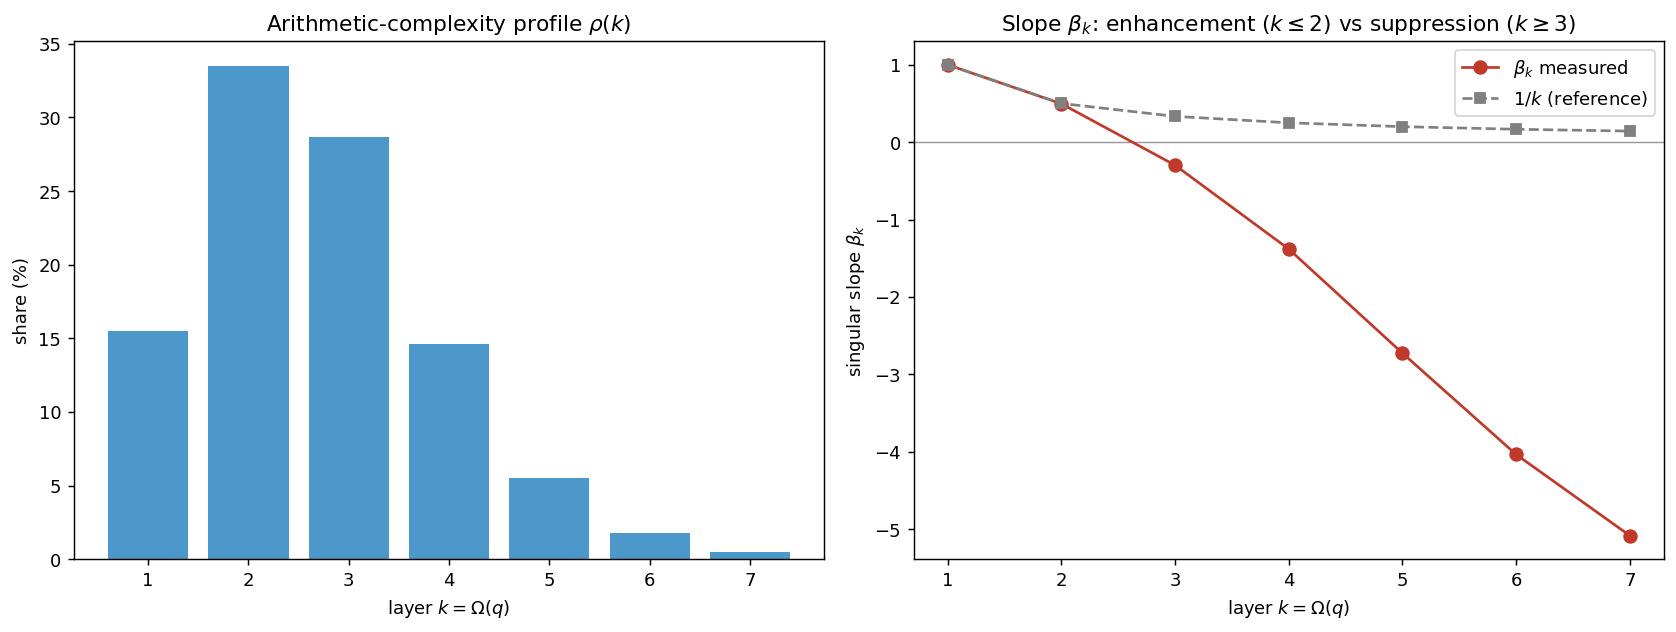
\includegraphics[width=\linewidth]{10_capas.png}
\caption{Left: the arithmetic-complexity profile $\rho(k)$ peaks at $k=2$. Right:
the singular exponent $\beta_k$ decreases through $1,\tfrac12,\dots$ and becomes
negative for $k\ge3$, diverging from the naive $1/k$ reference.}
\label{fig:layers}
\end{figure}

\paragraph{Sign reversal of the singular response.}
The Goldbach singular series \emph{enhances} the low-complexity channels
($\beta_1=1$, $\beta_2\approx\tfrac12>0$) but \emph{suppresses} the high-complexity
ones ($\beta_k<0$ for $k\ge3$): where $\sing(N)$ is large, representations with a
many-factored $q$ become rarer. The mechanism is the same divisor effect seen for
$R_2$, now run in reverse. When $\sing(N)$ is large, $N$ is divisible by many small
primes; the admissible $p$ avoid those residues, which forces $q=N-p$ to also avoid
small prime factors, so $q$ tends to have \emph{fewer} prime factors. Thus a large
singular series biases $q$ toward low arithmetic complexity. All $\beta_k$ drift
upward with $X$ at the same slow rate as $\beta_2$ (e.g.\ $\beta_3$ moves from
$-0.30$ at $2\cdot10^{6}$ to $-0.20$ at $8\cdot10^{6}$), so the crossing point of
$\beta_k=0$ moves slowly to the right. We also find that the strongest
``rescue'' channel, $q=$ composite$\times$composite (both factors composite), is
available for \emph{every} even $N$ in the range with on average $\sim1.8\cdot10^{4}$
representations: the additive hierarchy is extremely redundant below the prime
layer.

\subsection{Diagnostics}
\label{sec:diag-emp}

The prime share has mean $\bar\theta=0.311$ and decreases slowly with $N$ (the
semiprime channel gains ground, as the $\log\log N$ factor predicts); the Chen
surplus has mean $\overline{C}=2.27$. Goldbach fragility is extremely rare:
$|\mathcal F_1|=1$, $|\mathcal F_2|=3$, $|\mathcal F_3|=5$, $|\mathcal F_5|=14$,
$|\mathcal F_{10}|=49$ up to $X$; and \emph{every} fragile integer observed has
$R_2>0$, so Chen always rescues. The semiprime factor balance $B(q)=\log a/\log q$
has weighted mean $0.25$, with $16\%$ of the representation mass at $B<0.1$ (a tiny
prime factor) and $18\%$ at $B>0.4$ (near balanced): Chen representations are
dominated by \emph{unbalanced} semiprimes with a small prime factor
(Fig.~\ref{fig:balance}), answering Question~3.

\begin{figure}[h]
\centering
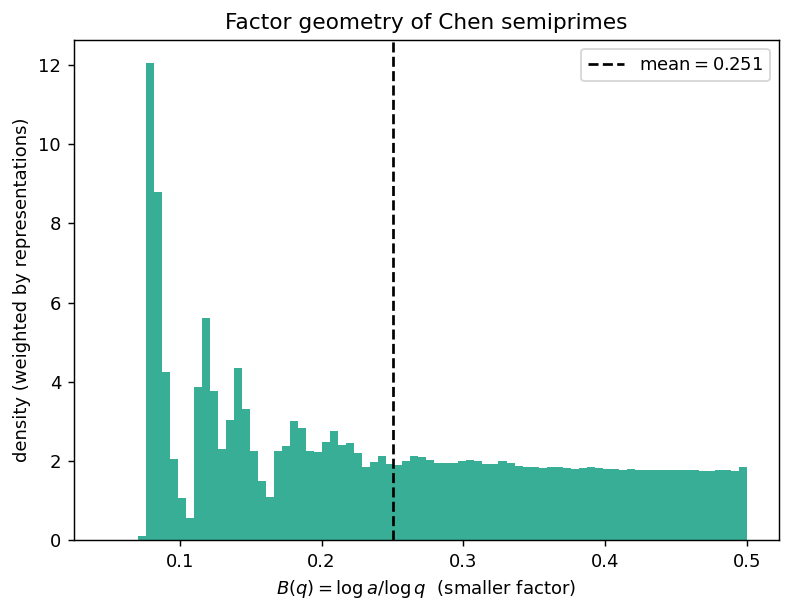
\includegraphics[width=0.62\linewidth]{05_balance.png}
\caption{Representation-weighted distribution of the factor balance $B(q)$ of the
semiprime second summand. Mass concentrates toward small $B$ (small prime factor),
not toward the balanced value $1/2$.}
\label{fig:balance}
\end{figure}

\subsection{Optimization experiments}

\paragraph{Smoothness is a Pareto trade-off.}
Minimizing the total spatial variation $\sum|s_N-s_{N-2}|$ of the selected location
$s_N=q_N/N$ yields a geometrically very smooth branch (total variation $0.0040$ over
$201$ consecutive even integers) that nonetheless \emph{switches type in $28\%$ of
its steps} and uses semiprimes $72\%$ of the time (Fig.~\ref{fig:branch}). Forbidding
semiprimes (the pure Goldbach branch, with zero type switches) raises the variation
to $0.0246$, a factor of $6.2$ rougher. One cannot simultaneously maximize geometric
and type smoothness: continuity in location and chaos in type coexist.

\begin{figure}[h]
\centering
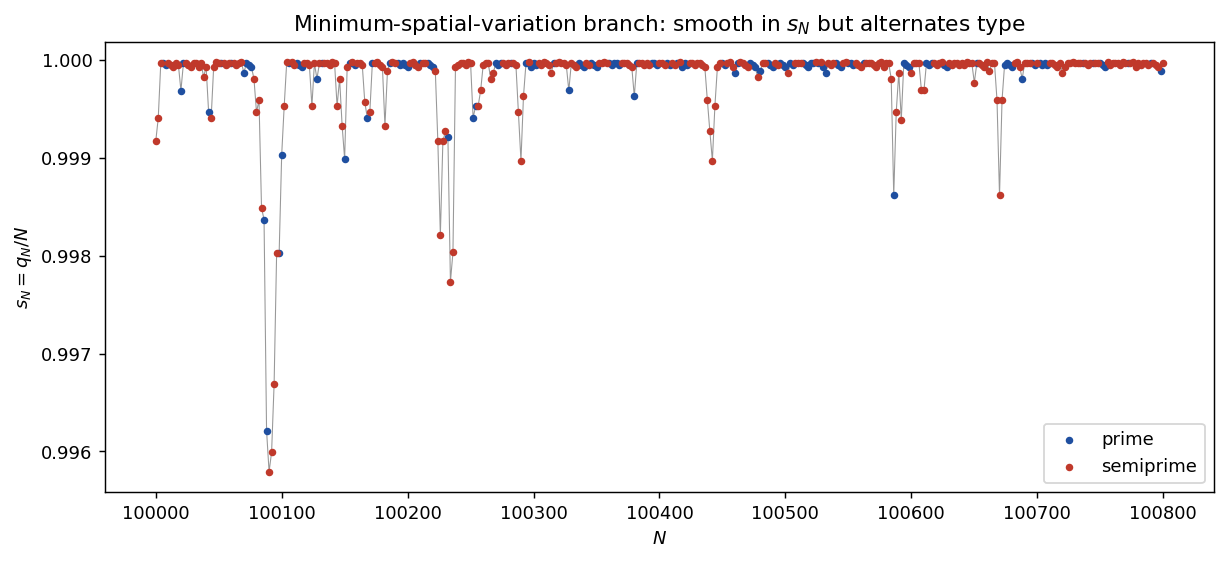
\includegraphics[width=\linewidth]{07_rama_mip.png}
\caption{Minimum-variation branch (Gurobi). The optimum hugs $s_N\approx1$ (the
``least partner'' branch, $p$ a small prime) and is smooth in $s_N$, yet its type
(blue prime / red semiprime) alternates.}
\label{fig:branch}
\end{figure}

\paragraph{A unimodal Chen-rescue threshold.}
Restricting representations to a balanced band $p\in[N/2-k,\,N/2]$ and measuring the
fraction of $N$ that \emph{require} a semiprime (no prime pair in the band) gives a
unimodal curve in $k$ (Fig.~\ref{fig:rescue}). For $k\gtrsim0.005\,N$ the prime
channel essentially never fails; the rescue fraction peaks near $38$--$40\%$ at an
intermediate half-width $k\sim20$--$40$; and for $k=1,2$ it falls again because
often no representation exists at all. The peak shifts right with $N$ (roughly as
$\log^2N$), marking where the expected number of balanced prime pairs,
$\sim2C_2\,\sing(N)\,k/\log^2(N/2)$, drops to $O(1)$ -- a Poisson-type transition.
This realizes the phase-diagram value $a_X^*(N)$ of \S12.1: Chen's semiprime
flexibility becomes \emph{necessary} precisely when near-perfect balance is imposed.

\begin{figure}[h]
\centering
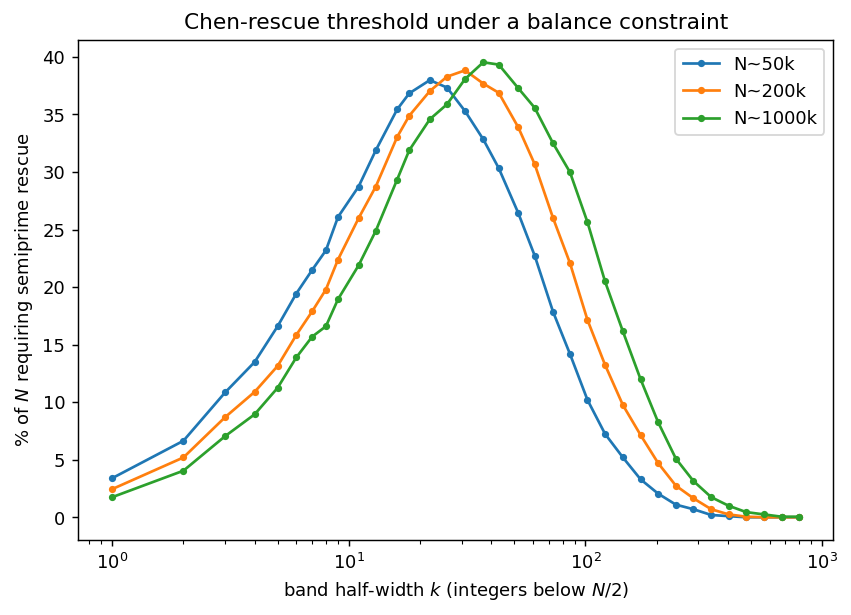
\includegraphics[width=0.7\linewidth]{06_rescate.png}
\caption{Fraction of $N$ that require a semiprime rescue as a function of the band
half-width $k$, for three scales of $N$. The curve is unimodal and its peak scales
like $\log^2N$.}
\label{fig:rescue}
\end{figure}

\subsection{Weak continuity of the location measures}

Finally we test the weak-continuity intuition of \S4 (Question~1 and
Conjecture~3) directly. The pointwise measure $\mu_N$ of $q/N$ is noisy, but
averaging over a window $N\in[X,X+H]$ produces a stable density
(Fig.~\ref{fig:continuity}, left). Three findings, at $X=10^{6}$:

\begin{itemize}[leftmargin=2em]
\item \textbf{The smoothed measure converges.} Splitting a window into two
same-scale subsamples, the total-variation distance between their densities falls
monotonically from $2.1\cdot10^{-3}$ to $3\cdot10^{-4}$ as $H$ grows from $125$ to
$4000$ (Fig.~\ref{fig:continuity}, right), i.e.\ the per-$N$ noise averages out --
a concrete form of weak convergence.
\item \textbf{The limit is essentially uniform.} The prime-$q$ density is within
total variation $0.028$ of the uniform law on $(0,1)$, with only a mild upturn near
the endpoints (the $1/(\log(xN)\log((1-x)N))$ effect). This answers Question~1
affirmatively: after removing endpoint effects, $\mu_N^{(1)}$ is close to uniform.
\item \textbf{Prime and semiprime locations nearly coincide.} The two densities are
within total variation $0.019$ of each other (Fig.~\ref{fig:continuity}, center),
confirming Conjecture~3. The semiprime location is slightly skewed toward larger
$q$ (mean $q/N=0.513$ versus the exactly symmetric $0.500$ for primes), the only
visible signature that $p$ and $q$ play asymmetric roles in $R_2$.
\end{itemize}

\begin{figure}[h]
\centering
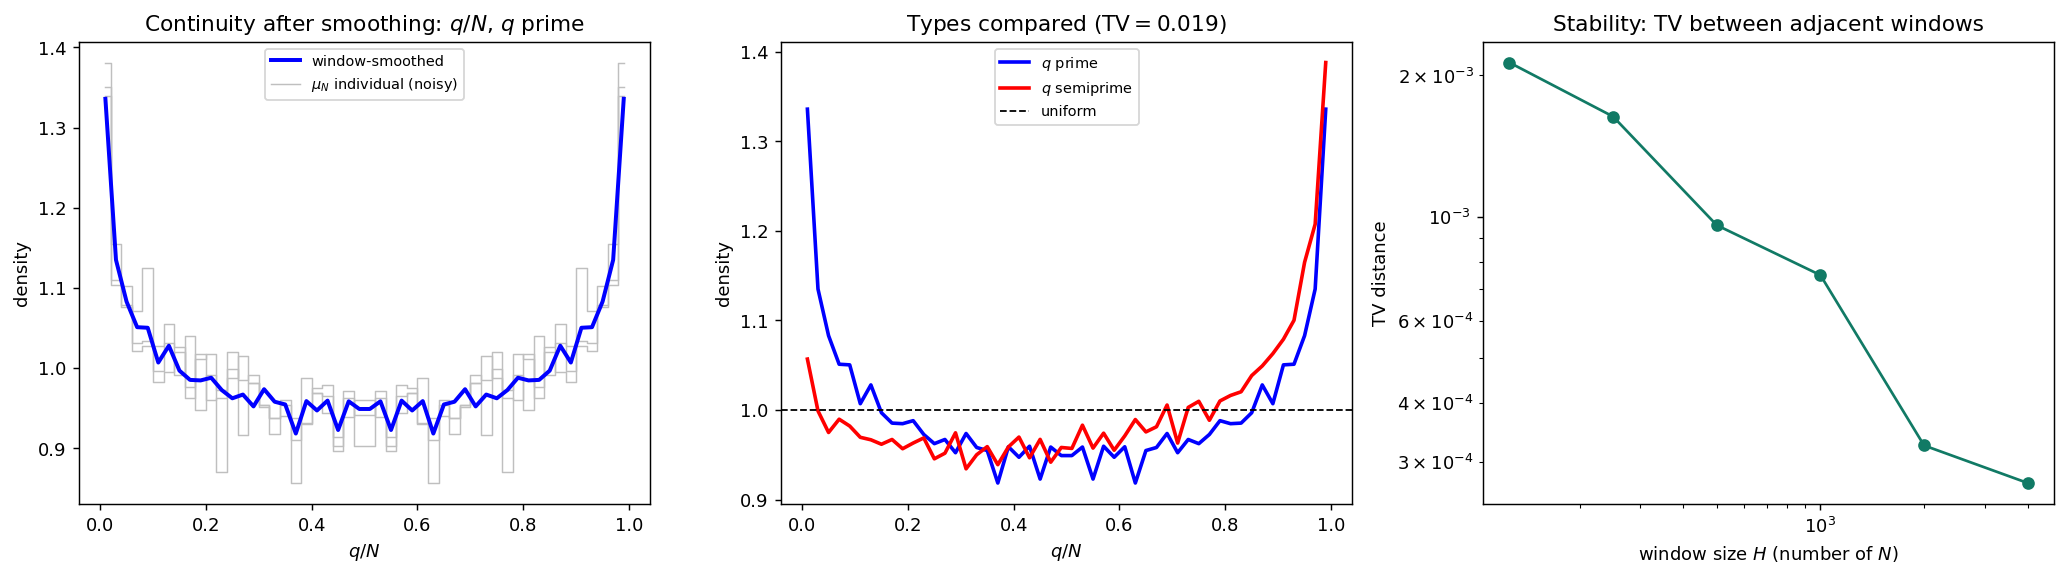
\includegraphics[width=\linewidth]{08_continuidad.png}
\caption{Weak continuity of $q/N$. Left: noisy pointwise $\mu_N$ (gray) versus the
window-smoothed density (blue). Center: prime versus semiprime location densities,
both close to uniform. Right: same-scale sampling distance decreases with the
window size $H$ (log--log).}
\label{fig:continuity}
\end{figure}

\subsection{The residual Goldbach--Chen balance exponent}
\label{sec:balance-emp}

Inspired by the $(1+a)$ interpolation of Li and Liu (every large even $N$ is
$p+rq$ with $r\le q^{a-1}$, so that $(1+1)$ is Goldbach and $(1+2)$ is Chen), one
can ask not whether a \emph{fixed} exponent works, but the smallest exponent
\emph{needed} for each $N$. For the nondegenerate Chen layer $N=p+rs$ ($p,r,s$
prime, $r\le s$), define the residual balance exponent and minimal multiplier
\[
  a_{\rm Res}(N)=1+\min_{N=p+rs}\frac{\log r}{\log s},
  \qquad
  r_\star(N)=\min\{r\in\PP:\exists\,p,s\in\PP,\ N=p+rs\}.
\]
We compute both exactly for all even $N\le2\cdot10^{6}$ ($r_\star$ by FFT channel
coverage; $a_{\rm Res}$ by a small-$p$ scan, validated against full enumeration to
$0$ error). Findings (Fig.~\ref{fig:balexp}, $N\ge1000$):

\begin{itemize}[leftmargin=2em]
\item \textbf{Typical residual collapse.} The median $a_{\rm Res}$ \emph{decreases}
with $X$ ($1.115\to1.099\to1.088$ at $X=10^5,5\cdot10^5,2\cdot10^6$), with
$p_{99}=1.182$ and a finite-range maximum of $1.385$ -- far below the Li--Liu
threshold $1.9$. The worst case is pinned by a few small ``hard'' $N$.
\item \textbf{The minimal multiplier is tiny.} $r_\star=3$ for $68\%$ of $N$ and the
dictionary $\{2,3,5,7\}$ already covers $99.7\%$; $\{2,\dots,11\}$ covers
$99.99\%$. This settles the multiplier-dictionary question empirically.
\item \textbf{Local obstruction.} $r_\star$ jumps when a small prime divides $N$: if
$3\mid N$ the channel $r=3$ is blocked (then $p=N-3s\equiv0\bmod3$), and indeed the
mean $r_\star$ is $4.59$ for $3\mid N$ versus $2.94$ otherwise.
\item \textbf{Link to the singular series.} $a_{\rm Res}$ correlates
\emph{positively} with $\log\sing(N)$ (correlation $+0.59$). The very divisibility
of $N$ by small primes that enlarges $\sing(N)$ (boosting Goldbach) also blocks the
small-$r$ Chen channels, so the residual balance is \emph{worst exactly where
Goldbach is locally richest}. This ties the balance exponent to the singular-series
theme of \S\ref{sec:layers-emp}.
\end{itemize}

\begin{figure}[h]
\centering
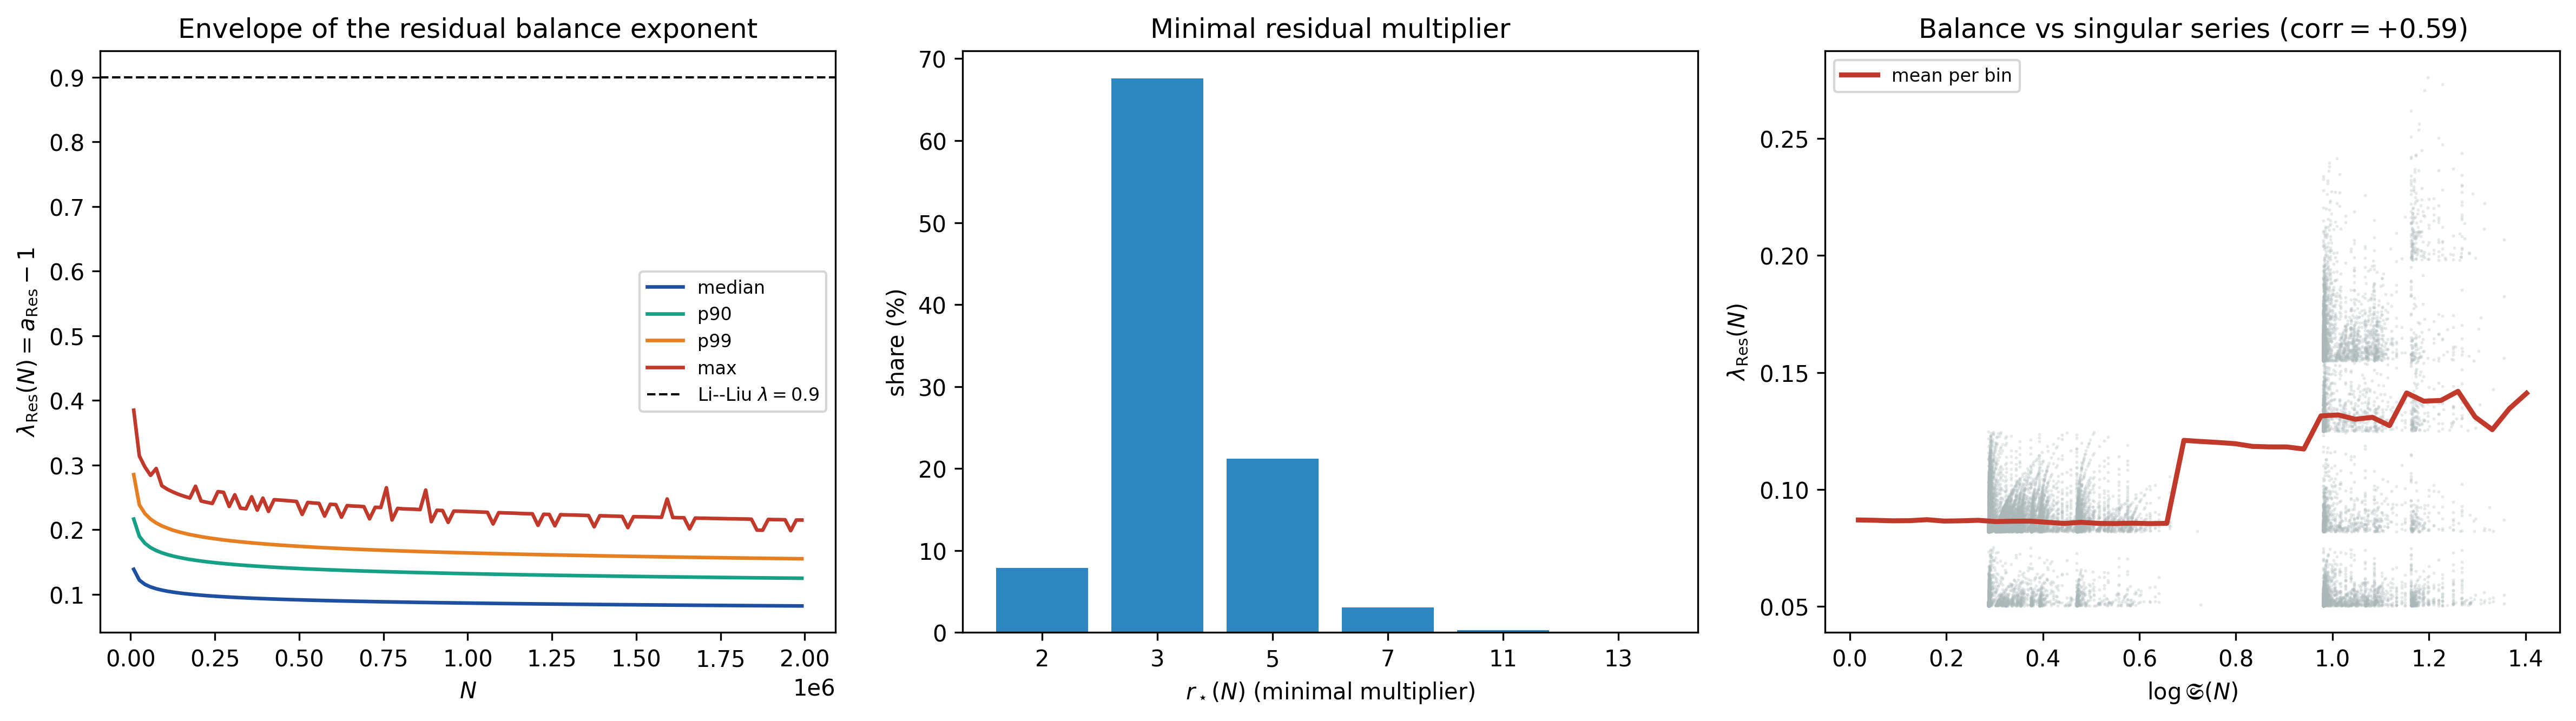
\includegraphics[width=\linewidth]{11_balance.png}
\caption{Left: percentile envelope of $\lambda_{\rm Res}=a_{\rm Res}-1$ versus $N$,
far below the Li--Liu line $0.9$. Centre: the minimal multiplier $r_\star$ ($r=3$
dominates). Right: $\lambda_{\rm Res}$ rises with the Goldbach singular series
$\sing(N)$ (positive correlation).}
\label{fig:balexp}
\end{figure}

\section{Conclusion}

The proposed project reframes the gap between Goldbach and Chen as an empirical and optimization-theoretic object. The key move is to distinguish prime--prime representations from prime--semiprime representations and then study their distribution, stability, and selectable smoothness. The infinite MIP formulation gives a formal covering interpretation of the conjectures, while the finite MIP creates new computational diagnostics: minimum semiprime use, minimum type switching, and minimum spatial variation. Finally, the weak-convergence formulation gives a precise way to express the intuition that the discrete representation function may look continuous only after normalization and smoothing.

This is not a proof of Goldbach. It is a research program that can produce reproducible computations, new empirical regularities, and potentially publishable questions at the boundary between additive number theory, computational experimentation, and discrete optimization.


\begin{thebibliography}{99}

\bibitem[Chen(1973)]{chen1973}
Chen, J. R. (1973).
\newblock On the representation of a larger even integer as the sum of a prime and the product of at most two primes.
\newblock \emph{Scientia Sinica}, 16, 157--176.

\bibitem[Helfgott(2014)]{helf2014ternary}
Helfgott, H. A. (2014).
\newblock The ternary Goldbach problem.
\newblock \emph{arXiv preprint arXiv:1404.2224}.

\bibitem[Landau(1909)]{landau1909}
Landau, E. (1909).
\newblock \emph{Handbuch der Lehre von der Verteilung der Primzahlen}.
\newblock Teubner.

\bibitem[Li and Liu(2026)]{li2026}
Li, J. and Liu, J. (2026).
\newblock Theorem $(1+1.9)$ on the Goldbach Conjecture.
\newblock \emph{arXiv preprint arXiv:2606.05224}.

\bibitem[Montgomery and Vaughan(1975)]{montgomeryvaughan1975}
Montgomery, H. L. and Vaughan, R. C. (1975).
\newblock The exceptional set in Goldbach's problem.
\newblock \emph{Acta Arithmetica}, 27, 353--370.

\bibitem[Nathanson(1996)]{nathanson}
Nathanson, M. B. (1996).
\newblock \emph{Additive Number Theory: The Classical Bases}.
\newblock Springer.

\bibitem[Oliveira e Silva et al.(2014)]{silva2014}
Oliveira e Silva, T., Herzog, S., and Pardi, S. (2014).
\newblock Empirical verification of the even Goldbach conjecture and computation of prime gaps up to $4\cdot10^{18}$.
\newblock \emph{Mathematics of Computation}, 83(288), 2033--2060.

\bibitem[Hardy and Wright(2008)]{hardywright}
Hardy, G. H. and Wright, E. M. (2008).
\newblock \emph{An Introduction to the Theory of Numbers}.
\newblock Oxford University Press, 6th edition.

\end{thebibliography}

\end{document}
